\chapter{Lecture Notes}
\setlength{\headheight}{12.71342pt}
\addtolength{\topmargin}{-0.71342pt}

\section{1\texorpdfstring{\textsuperscript{st}}{st} Lecture - Plants and Food Colours}
\subsection*{Lecture Goals}
After this lecture, the students will be able to:
\begin{highlight}
    \begin{itemize}
    \item Describe the structures of fruits and vegetables
    
    \item Identify structural carbohydrates in plants \& changes they undergo during ripening and processing
    
    \item Describe important factors responsible for texture, colours, flavours, and taste of plants
    \end{itemize}
\end{highlight}

\subsection*{Plant Organs}
Plants have different organs, each serving a specific function. Table \ref{tab:L01_plant_organs} shows some plant organs and examples of fruits and vegetables which has the following trait.
\begin{table}[ht]
    \centering
    \caption{A table showing plant organs and examples}
    \label{tab:L01_plant_organs}
    \begin{tabular}{|p{1.9cm}|p{3cm}|p{6cm}|p{3cm}|}
    \hline
    \textbf{Organ} & \textbf{Function} & \textbf{Plant material and cell type} & \textbf{Example} \\
    \hline
    \multirow{2}{3cm}{Roots} & Anchor plants into ground, absorb nutrients & Tough fibrous material -- cells have thick, cellulose-rich cell walls.  & Inedible \\
    \cline{3-4}
    & & Some roots swell up with storage cells full of \textit{amyloplasts} & Carrots, parsnips, radishes, sweet po-tatoes \\
    \hline
    \multirow{2}{3cm}{Stems, stalks} & Conduct nutrients to roots and leaves, gives structural support & Fibrous material (stems, stalks) - cells have thick, cellulose-rich cell walls & Asparagus stems, cellery stalks \\
    \cline{1-1} \cline{3-4}
    Tubers, rhizomes & & Some stems swell up with storage tissue (tubers rhizomes) -cells are full with \textit{amyloplasts} & Potato, turnip, ginger \\
    \hline
    Leaves & Produce sugar molecules by photosynthesis & Plant material is thin so gases can penetrate/escape. Almost no structural support—cell walls are thin and flexible. Cells have many chloroplasts and large air pockets between them for gases. & Spinach leaves, lettuce leaves \\
    \hline
    Flowers & Reproduction & Contain reproductive organs, Often colorful to attract pollinators & Cauliflower, broccoli \\
    \hline
    Fruits & Seed dispersal & Fleshy or dry structures, Contain seeds & Apples, oranges \\
    \hline
    Seeds & Germination & Contain embryo and nutrients, Protected by seed coat & Peas, beans \\
    \hline
    \end{tabular}
\end{table}

\subsection*{Hemicelluloses}
\begin{itemize}
    \item Hemicelluloses contain a variety of sugars in their long
    chains—unlike starch and cellulose
    \subitem They contain both pentoses and hexoses
    
    \item Hemicelluloses, matted with pectic substances, serve as a
    connection between fibrillar cellulose
    
    \item Alkaline medium has a strong effect—vegetables cooked
    with baking soda added become flaccid \& mushy
    \subitem Baking soda also has a destructive effect on thiamine
\end{itemize}

\vspace{0.5em}
Xylan and arabinan are two particularly common hemicelluloses with
glucuronic acid attached, which is a common feature of pectic. Figure \ref{fig:L01_hemicelluloses} shows the structure of these.
\begin{figure}[ht]
    \centering
    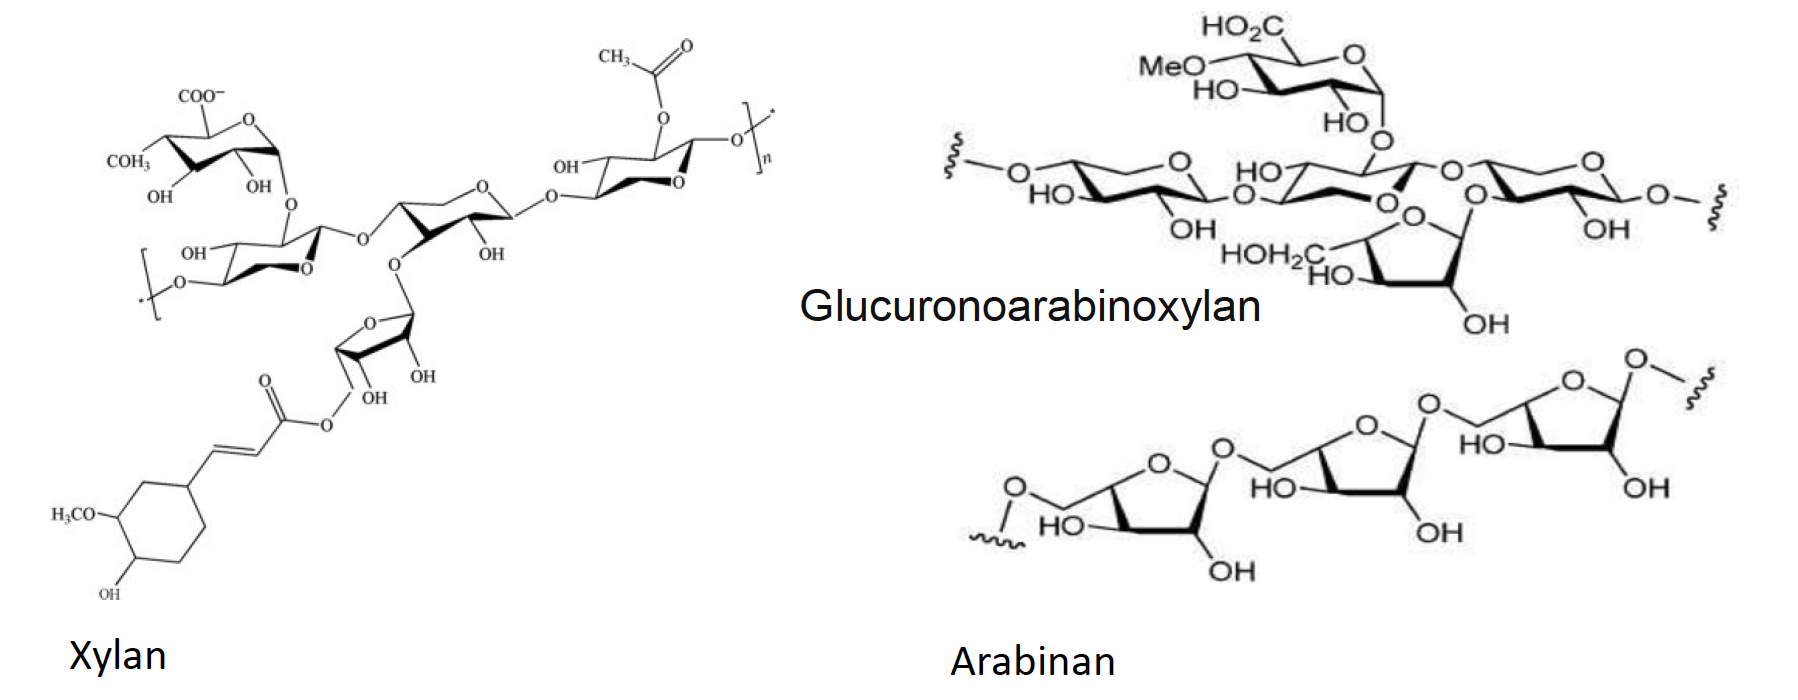
\includegraphics[width=\textwidth]{figures/L01_hemicelluloses.png}
    \caption{Structure of hemicelluloses}
    \label{fig:L01_hemicelluloses}
\end{figure}

\subsection*{Pectic Substances}

\begin{itemize}
    \item Pectic substances is a general term for member
    of this family of polygalacturonic acid compounds
    \subitem Protopectin, pectin and pectic acid
    
    \item Contained in the primary cell wall and the middle lamella (the
    outer region of the cell wall)
    
    \item Pectic substances in the middle lamella change form during the
    maturation process
    
    \item Combine with hemicellulose in the primary cell wall to form the
    "cement" surrounding the cellulose fibers
\end{itemize}

\vspace{0.5em}
Protopectin is water-insoluble, and occurs in immature fruits and, to a lesser extent, in vegetables. Pectin is water-soluble, and is found in ripe fruits and vegetables. Pectic acid is formed when pectin is heated in an acid medium. Figure \ref{fig:L01_propectin} shows the structure of these.

\begin{figure}[h]
    \centering
    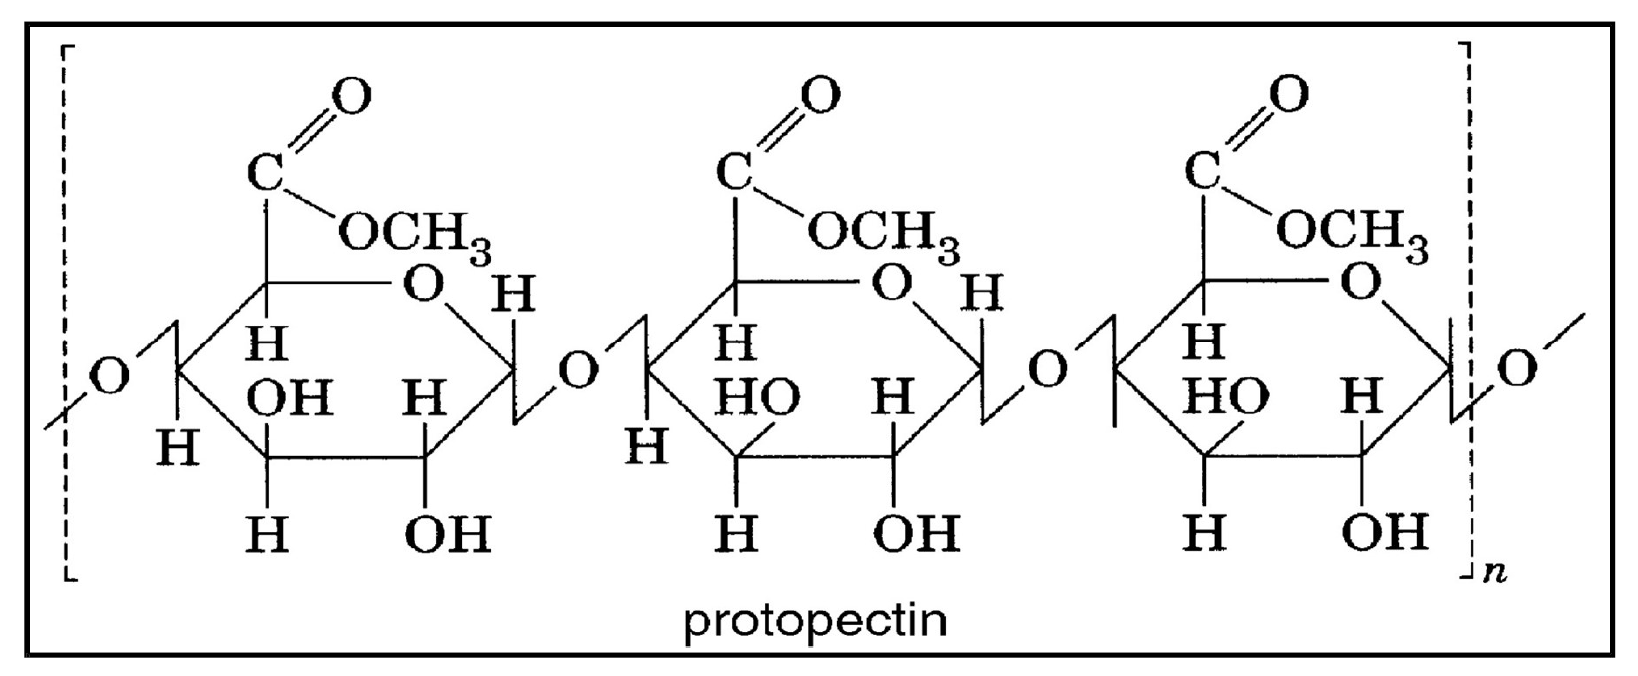
\includegraphics[width=0.7\textwidth]{figures/L01_propectin.png}
    \caption{This form is a methylated (methyl ester groups), very long polymer of galacturonic acid}
    \label{fig:L01_propectin}
\end{figure}

\subsection*{Starchy Vegetables and Texture}
When vegetables are raw, their starch granules are hard and give a chalky feeling when chewed. When cooked, the starch granules begin to soften around 60\textdegree C, when cell membranes are also affected. Starch granules absorb water which disrupt their structure and they swell, forming a gel. Vegetables becomes tender but dry. When cell walls are weak, the gel-filled cells pull away from each other as separate particles giving a mealy impression.

\subsubsection*{Important Factors During Precessing of Potatoes}

\begin{highlight}
    \begin{itemize}
        \item Boiling - Pectin crosslinking promoted by enzyme activity at 55-60\textdegree C for 20-30 min
        \subitem Firm potato. According to McGee, enzyme in the cell wall alters cell well pectins - more easily cross-linked by calcium ions (activated around 50\textdegree C and inactivated around 70\textdegree C)
        \item Frying - Starch leaks out of granules and glues outer cell walls together when initial frying temperature is kept low (120-160\textdegree C) - crisp crust
        \item Grayish discolouration: caused by a pigmented complex formed by chlorogenic acid, oxygen and iron ions
        \subitem Minimized at low pH
        \item Leftover potatoes get a stale, cardboard flavour, due to membrane lipids being oxidized
        \item Salt speeds up softening (Sodium ions destabilize cell wall)
        \item Ca$^2$ slows down softening (stabilizes cell wall)
        \item High pH soften hemicellulose and open starch structure
    \end{itemize}
\end{highlight}

\section{2\texorpdfstring{\textsuperscript{nd}}{nd} Lecture - Carbohydrates I}
\subsection*{Carbohydrates in food}
In foods various carbohydrates are present. Some examples are listed in Table \ref{tab:L02_carbohydrates}.
\begin{table}[ht]
    \centering
    \caption{Carbohydrates in food with classification based on their molecular size}
    \label{tab:L02_carbohydrates}
    \rowcolors{1}{gray!7}{white}
    \begin{tabular}{l|l|l|l}
    \textbf{Monosaccharides} & \textbf{Di-} & \textbf{Oligo-} & \textbf{Poly-} \\
    \hline
    Glucose & Sucrose & \textbf{Digestible:} & \textbf{Digestible:} \\

    Fructose & Lactose & Maltotriose & Starch \\

    Galactose & Maltose & Maltotetrose & (Amylose, amylopectin) \\

    Mannose & Cellobiose & Maltopentose & \\

    Ribose & Trehalose & \textbf{Non-digestible} & \textbf{Non-digestible} \\

    Xylose & ... & Rafinose & \underline{Soluble:} agar, gum arabic, carrageenan, pectin, ... \\
    ... & & Starchyose & \underline{Insoluble:} cellulose, protopectin, chitin, ... \\
    \end{tabular}
\end{table}

\subsection*{Anomeric Carbon and Reducing Sugar}
The anomeric carbon originates from the carbonyl group in the open-chain form of a sugar and becomes a stereocenter in the cyclic form, capable of forming alpha and beta isomers. Reducing sugars can switch back to the open-chain form, exposing the reactive carbonyl group, key in reactions like the Maillard reaction. Non-reducing sugars, like sucrose, have their anomeric carbon locked, preventing such reactivity. An example of an open-chain and cyclic form of a monosaccharide is shown in Figure \ref{fig:L02_anomeric_carbon} where the anomeric carbon is highlighted in red. The term "masked oxo-group" refers to the carbonyl group (C=O) in the open-chain form being hidden in the ring structure.
\begin{figure}[h]
    \centering
    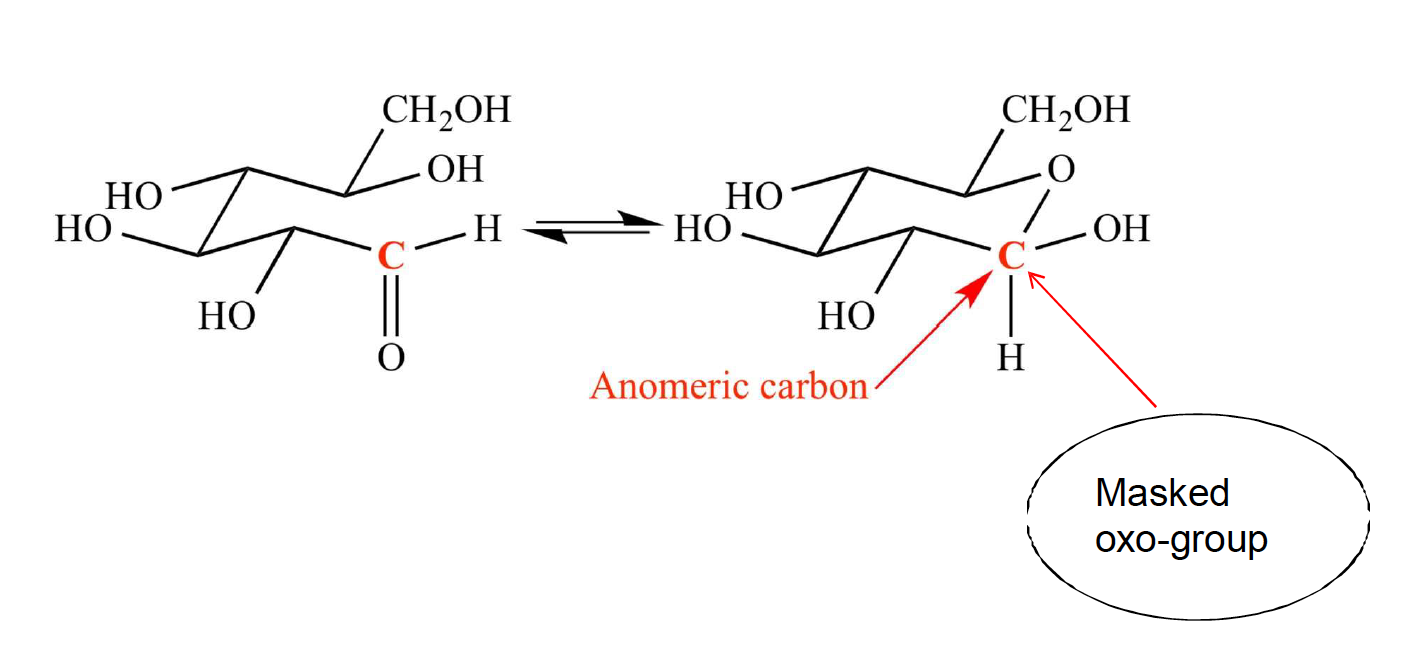
\includegraphics[width=0.7\textwidth]{figures/L02_anomeric_carbon.png}
    \caption{An example of an open-chain and cyclic form of a monosaccharide}
    \label{fig:L02_anomeric_carbon}
\end{figure}


\section{12\texorpdfstring{\textsuperscript{th}}{th} Lecture - Stocks and Sauces}


